% Source PDF page 575 (printed p. 561)
\section{不等式约束最小化问题}
本章讨论求解含不等式约束的凸优化问题的内点法：
\begin{equation}\begin{aligned}
\text{最小化}\quad &f_0(x)\\
\text{约束为}\quad &f_i(x)\le0,\quad i=1,\ldots,m,\\
&Ax=b,
\end{aligned}\tag{11.1}\end{equation}
其中 $f_0,\ldots,f_m:\R^n\to\R$ 为凸且二阶连续可微函数，$A\in\R^{p\times n}$，并且 $\rank A=p<n$。假设该问题可解，即存在最优解 $x^\star$，以 $p^\star$ 表示最优值 $f_0(x^\star)$。

还假设该问题严格可行，即存在 $x\in\mathcal D$，满足 $Ax=b$ 以及 $f_i(x)<0$，$i=1,\ldots,m$。这意味着 Slater 约束资格条件成立，因而存在对偶最优解 $\lambda^\star\in\R^m$、$\nu^\star\in\R^p$，它们与 $x^\star$ 一起满足 KKT 条件
\begin{equation}\begin{aligned}
Ax^\star&=b,\qquad f_i(x^\star)\le0,\quad i=1,\ldots,m,\\
\lambda^\star&\succeq0,\\
\nabla f_0(x^\star)+\sum_{i=1}^m\lambda_i^\star\nabla f_i(x^\star)+A^\T\nu^\star&=0,\\
\lambda_i^\star f_i(x^\star)&=0,\quad i=1,\ldots,m.
\end{aligned}\tag{11.2}\end{equation}
内点法将牛顿法应用于一系列等式约束问题，或一系列修改后的 KKT 条件，从而求解问题 (11.1)（或 KKT 条件 (11.2)）。我们将重点讨论一种具体的内点算法——障碍法，并给出其收敛性证明与复杂度分析。还将在第11.7节介绍一种简单的原始—对偶内点法，但不作分析。

可以把内点法看作凸优化算法层次中的又一层。最简单的是线性等式约束二次问题。对这类问题，KKT 条件是一组线性方程，可以解析求解。牛顿法处于下一层。可以认为，牛顿法通过将具有二阶可微目标函数的线性等式约束优化问题化为一系列线性等式约束二次问题，来求解前者。
% Source PDF page 576 (printed p. 562)
内点法则再进一层：它将带有线性等式约束和不等式约束的优化问题，化为一系列线性等式约束问题来求解。

\subsection*{例子}
许多问题已经具有 (11.1) 的形式，而且满足目标函数与约束函数二阶可微的假设。明显的例子包括 LP、QP、QCQP 以及凸形式的 GP；另一个例子是带线性不等式约束的熵最大化问题，
\[
\begin{aligned}
\text{最小化}\quad&\sum_{i=1}^n x_i\log x_i\\
\text{约束为}\quad&Fx\preceq g,\\
&Ax=b,
\end{aligned}
\]
其定义域为 $\mathcal D=\R_{++}^n$。

另外许多问题并不具有要求的 (11.1) 形式，其目标函数和约束函数也不是二阶可微的，但可以重新表述成所需形式。我们已经见过许多这样的例子，例如，将无约束凸分段线性最小化问题
\[
\text{最小化}\quad\max_{i=1,\ldots,m}(a_i^\T x+b_i)
\]
（其目标函数不可微）转化为 LP
\[
\begin{aligned}
\text{最小化}\quad&t\\
\text{约束为}\quad&a_i^\T x+b_i\le t,\quad i=1,\ldots,m
\end{aligned}
\]
（其目标函数和约束函数都是二阶可微的）。

有些凸优化问题，例如 SOCP 和 SDP，不容易改写为所需形式，但可以用处理广义不等式问题的内点法扩展来求解。第11.6节将介绍这种扩展。

\section{对数障碍函数与中心路径}
我们的目标是把不等式约束问题 (11.1) 近似表述为可应用牛顿法的等式约束问题。第一步是将不等式约束隐含在目标函数中，把问题 (11.1) 改写为
\begin{equation}\begin{aligned}
\text{最小化}\quad&f_0(x)+\sum_{i=1}^m I_-(f_i(x))\\
\text{约束为}\quad&Ax=b,
\end{aligned}\tag{11.3}\end{equation}
其中 $I_-:\R\to\R$ 是非正实数集的示性函数：
\[
I_-(u)=\begin{cases}0,&u\le0,\\\infty,&u>0.\end{cases}
\]
% Source PDF page 577 (printed p. 563)
\begin{figure}[htbp]\centering
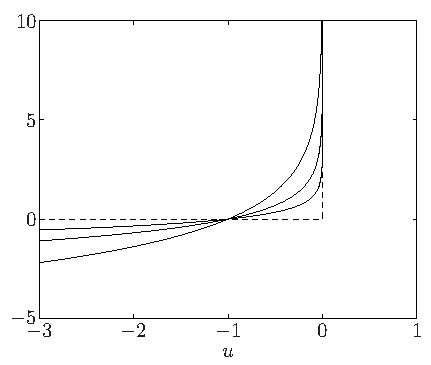
\includegraphics[width=.55\textwidth]{figures/ch11-01.pdf}
\caption*{图11.1 虚线表示函数 $I_-(u)$，实线表示 $\widehat I_-(u)=-(1/t)\log(-u)$，其中 $t=0.5,1,2$。$t=2$ 对应的曲线给出最好的近似。}
\end{figure}
问题 (11.3) 没有不等式约束，但其目标函数一般不可微，因此不能应用牛顿法。

\subsection{对数障碍}
障碍法的基本思想是用函数
\[
\widehat I_-(u)=-(1/t)\log(-u),\qquad\dom\widehat I_-=-\R_{++}
\]
近似示性函数 $I_-$，其中参数 $t>0$ 决定近似的精度。与 $I_-$ 一样，$\widehat I_-$ 为凸且非减函数，并且按照我们的约定，当 $u>0$ 时取值为 $\infty$。但是，$\widehat I_-$ 与 $I_-$ 不同，它可微且为闭函数：当 $u$ 增大趋近 $0$ 时，它增大趋于 $\infty$。图11.1给出了函数 $I_-$ 以及若干 $t$ 值下的近似 $\widehat I_-$。$t$ 越大，近似越准确。

在 (11.3) 中用 $\widehat I_-$ 替代 $I_-$，得到近似问题
\begin{equation}\begin{aligned}
\text{最小化}\quad&f_0(x)-\frac1t\sum_{i=1}^m\log(-f_i(x))\\
\text{约束为}\quad&Ax=b.
\end{aligned}\tag{11.4}\end{equation}
这里的目标函数可微，而且为凸函数，因为 $-(1/t)\log(-u)$ 关于 $u$ 凸且递增。在适当的闭性条件成立时，可以用牛顿法求解。

函数
\begin{equation}
\phi(x)=-\sum_{i=1}^m\log(-f_i(x)),\tag{11.5}
\end{equation}
% Source PDF page 578 (printed p. 564)
其定义域为 $\dom\phi=\{x\in\R^n\mid f_i(x)<0,\ i=1,\ldots,m\}$，称为问题 (11.1) 的\emph{对数障碍函数}，简称对数障碍。其定义域由严格满足 (11.1) 中不等式约束的点组成。无论正参数 $t$ 取何值，只要任一 $f_i(x)\to0$，对数障碍就无界增长。

当然，问题 (11.4) 只是原问题 (11.3) 的近似，因此马上会遇到这样一个问题：(11.4) 的解在多大程度上近似原问题 (11.3) 的解？直观上，随着参数 $t$ 增大，近似质量应当改善，我们很快就会证实这一点。

另一方面，当参数 $t$ 很大时，函数 $f_0+(1/t)\phi$ 在可行集边界附近的 Hessian 矩阵变化迅速，使牛顿法难以最小化它。我们将看到，可以通过依次求解一系列 (11.4) 形式的问题来避开这一困难：每一步增大参数 $t$（从而提高近似精度），并以上一个 $t$ 值对应问题的解，作为下一次牛顿最小化的起点。

为便于后续引用，记下对数障碍函数 $\phi$ 的梯度与 Hessian 矩阵：
\begin{align*}
\nabla\phi(x)&=\sum_{i=1}^m\frac1{-f_i(x)}\nabla f_i(x),\\
\nabla^2\phi(x)&=\sum_{i=1}^m\frac1{f_i(x)^2}\nabla f_i(x)\nabla f_i(x)^\T
+\sum_{i=1}^m\frac1{-f_i(x)}\nabla^2 f_i(x)
\end{align*}
（见第A.4.2节与第A.4.4节）。

\subsection{中心路径}
现在更详细地考察最小化问题 (11.4)。将目标乘以 $t$，考虑具有相同最小化点的等价问题
\begin{equation}\begin{aligned}
\text{最小化}\quad&tf_0(x)+\phi(x)\\
\text{约束为}\quad&Ax=b,
\end{aligned}\tag{11.6}\end{equation}
这样可以简化后面的记号。暂时假设问题 (11.6) 可以用牛顿法求解，特别地，对每个 $t>0$ 都有唯一解。（第11.3.3节将更详细地讨论这个假设。）

对 $t>0$，定义 $x^\star(t)$ 为 (11.6) 的解。问题 (11.1) 的\emph{中心路径}定义为点 $x^\star(t)$（$t>0$）组成的集合，这些点称为\emph{中心点}。中心路径上的点可由如下充要条件刻画：$x^\star(t)$ 严格可行，即满足
\[
Ax^\star(t)=b,\qquad f_i(x^\star(t))<0,\quad i=1,\ldots,m,
\]
并且存在 $\widehat\nu\in\R^p$ 使得
% Source PDF page 579 (printed p. 565)
\begin{equation}\begin{aligned}
0&=t\nabla f_0(x^\star(t))+\nabla\phi(x^\star(t))+A^\T\widehat\nu\\
&=t\nabla f_0(x^\star(t))+\sum_{i=1}^m\frac1{-f_i(x^\star(t))}\nabla f_i(x^\star(t))+A^\T\widehat\nu
\end{aligned}\tag{11.7}\end{equation}
成立。

\begin{origexample}{11.1}
\emph{不等式形式的线性规划。} 对不等式形式的 LP
\begin{equation}\begin{aligned}
\text{最小化}\quad&c^\T x\\\text{约束为}\quad&Ax\preceq b,
\end{aligned}\tag{11.8}\end{equation}
其对数障碍函数为
\[
\phi(x)=-\sum_{i=1}^m\log(b_i-a_i^\T x),\qquad\dom\phi=\{x\mid Ax\prec b\},
\]
其中 $a_1^\T,\ldots,a_m^\T$ 是 $A$ 的各行。障碍函数的梯度与 Hessian 矩阵为
\[
\nabla\phi(x)=\sum_{i=1}^m\frac{a_i}{b_i-a_i^\T x},\qquad
\nabla^2\phi(x)=\sum_{i=1}^m\frac{a_i a_i^\T}{(b_i-a_i^\T x)^2},
\]
或更紧凑地写为
\[
\nabla\phi(x)=A^\T d,\qquad\nabla^2\phi(x)=A^\T\diag(d)^2A,
\]
其中 $d\in\R^m$ 的分量为 $d_i=1/(b_i-a_i^\T x)$。由于 $x$ 严格可行，有 $d\succ0$，因此 $\phi$ 的 Hessian 矩阵非奇异当且仅当 $A$ 的秩为 $n$。中心性条件 (11.7) 为
\begin{equation}
tc+\sum_{i=1}^m\frac{a_i}{b_i-a_i^\T x}=tc+A^\T d=0.\tag{11.9}
\end{equation}
中心性条件有一个简单的几何解释。在中心路径上的点 $x^\star(t)$ 处，梯度 $\nabla\phi(x^\star(t))$ 垂直于经过 $x^\star(t)$ 的 $\phi$ 的水平集，且必须与 $-c$ 平行。换言之，超平面 $c^\T x=c^\T x^\star(t)$ 与经过 $x^\star(t)$ 的 $\phi$ 的水平集相切。图11.2给出 $m=6$、$n=2$ 的一个例子。
\end{origexample}

\subsubsection*{由中心路径得到对偶点}
从 (11.7) 可以推导中心路径的一项重要性质：每个中心点都给出一个对偶可行点，因而给出最优值 $p^\star$ 的下界。具体而言，定义
\begin{equation}
\lambda_i^\star(t)=-\frac1{t f_i(x^\star(t))},\quad i=1,\ldots,m,
\qquad\nu^\star(t)=\widehat\nu/t.\tag{11.10}
\end{equation}
我们断言，点对 $\lambda^\star(t),\nu^\star(t)$ 对偶可行。

首先，由于 $f_i(x^\star(t))<0$，$i=1,\ldots,m$，显然 $\lambda^\star(t)\succ0$。将最优性条件 (11.7) 写为
\[
\nabla f_0(x^\star(t))+\sum_{i=1}^m\lambda_i^\star(t)\nabla f_i(x^\star(t))+A^\T\nu^\star(t)=0,
\]
% Source PDF page 580 (printed p. 566)
\begin{figure}[htbp]\centering
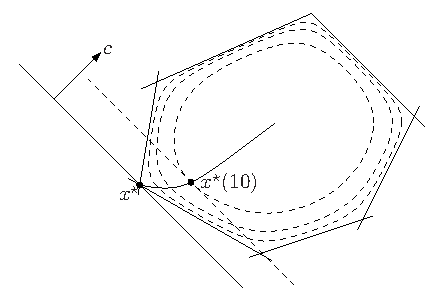
\includegraphics[width=.6\textwidth]{figures/ch11-02.pdf}
\caption*{图11.2 一个 $n=2$、$m=6$ 的 LP 的中心路径。虚线是对数障碍函数 $\phi$ 的三条等高线。随着 $t\to\infty$，中心路径收敛到最优点 $x^\star$。图中还标出了 $t=10$ 对应的中心路径上的点。在该点可以从几何上验证最优性条件 (11.9)：直线 $c^\T x=c^\T x^\star(10)$ 与经过 $x^\star(10)$ 的 $\phi$ 的等高线相切。}
\end{figure}
可见，当 $\lambda=\lambda^\star(t)$、$\nu=\nu^\star(t)$ 时，$x^\star(t)$ 最小化拉格朗日函数
\[
L(x,\lambda,\nu)=f_0(x)+\sum_{i=1}^m\lambda_i f_i(x)+\nu^\T(Ax-b),
\]
这说明 $\lambda^\star(t),\nu^\star(t)$ 是对偶可行点对。因此，对偶函数 $g(\lambda^\star(t),\nu^\star(t))$ 有限，且
\begin{align*}
g(\lambda^\star(t),\nu^\star(t))
&=f_0(x^\star(t))+\sum_{i=1}^m\lambda_i^\star(t)f_i(x^\star(t))
+\nu^\star(t)^\T(Ax^\star(t)-b)\\
&=f_0(x^\star(t))-m/t.
\end{align*}
特别地，$x^\star(t)$ 与对偶可行点对 $\lambda^\star(t),\nu^\star(t)$ 对应的对偶间隙就是 $m/t$。一个重要推论是
\[
f_0(x^\star(t))-p^\star\le m/t,
\]
即 $x^\star(t)$ 的次优程度不超过 $m/t$。这证实了如下直观认识：当 $t\to\infty$ 时，$x^\star(t)$ 收敛到一个最优点。

\begin{origexample}{11.2}
\emph{不等式形式的线性规划。} 不等式形式 LP (11.8) 的对偶为
\[
\begin{aligned}
\text{最大化}\quad&-b^\T\lambda\\
\text{约束为}\quad&A^\T\lambda+c=0,\\&\lambda\succeq0.
\end{aligned}
\]
从最优性条件 (11.9) 显然可见，
\[
\lambda_i^\star(t)=\frac1{t(b_i-a_i^\T x^\star(t))},\quad i=1,\ldots,m,
\]
% Source PDF page 581 (printed p. 567)
是对偶可行的，其对偶目标值为
\[
-b^\T\lambda^\star(t)=c^\T x^\star(t)+(Ax^\star(t)-b)^\T\lambda^\star(t)
=c^\T x^\star(t)-m/t.
\]
\end{origexample}

\subsubsection*{用 KKT 条件解释}
还可以把中心路径条件 (11.7) 看作 KKT 最优性条件 (11.2) 的连续变形。点 $x$ 等于 $x^\star(t)$ 当且仅当存在 $\lambda,\nu$ 使得
\begin{equation}\begin{aligned}
Ax&=b,\qquad f_i(x)\le0,\quad i=1,\ldots,m,\\
\lambda&\succeq0,\\
\nabla f_0(x)+\sum_{i=1}^m\lambda_i\nabla f_i(x)+A^\T\nu&=0,\\
-\lambda_i f_i(x)&=1/t,\quad i=1,\ldots,m.
\end{aligned}\tag{11.11}\end{equation}
KKT 条件 (11.2) 与中心性条件 (11.11) 的唯一区别，是将互补条件 $-\lambda_i f_i(x)=0$ 替换为 $-\lambda_i f_i(x)=1/t$。特别地，当 $t$ 很大时，$x^\star(t)$ 以及相应的对偶点 $\lambda^\star(t),\nu^\star(t)$ “几乎”满足 (11.1) 的 KKT 最优性条件。

\subsubsection*{力场解释}
可以用作用在严格可行集 $C$ 内一个质点上的势力，对中心路径作简单的力学解释。为简便起见，假设没有等式约束。

对每个约束，令它在质点位于 $x$ 时施加的力为
\[
F_i(x)=-\nabla(-\log(-f_i(x)))=\frac1{f_i(x)}\nabla f_i(x).
\]
所有约束产生的总力场对应的势为对数障碍 $\phi$。当质点向可行集边界移动时，会受到约束产生的强烈排斥力。

现在设质点在位置 $x$ 还受到另一个力
\[
F_0(x)=-t\nabla f_0(x).
\]
这个目标力场沿负梯度方向牵引质点，也就是使它向较小的 $f_0$ 移动。参数 $t$ 决定目标力相对于约束力的大小。

中心点 $x^\star(t)$ 就是约束力与质点所受目标力恰好平衡的位置。随着参数 $t$ 增大，质点被更强地牵向最优点，但它始终被障碍势限制在 $C$ 内，因为当质点接近边界时，障碍势变为无穷大。

\begin{origexample}{11.3}
\emph{不等式形式 LP 的力场解释。} 与 LP (11.8) 第 $i$ 个约束对应的力场为
\[
F_i(x)=\frac{-a_i}{b_i-a_i^\T x}.
\]
% Source PDF page 582 (printed p. 568)
\begin{figure}[htbp]\centering
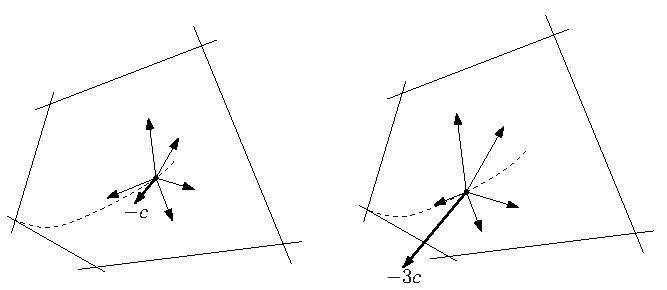
\includegraphics[width=.85\textwidth]{figures/ch11-03.pdf}
\caption*{图11.3 中心路径的力场解释。虚线表示中心路径。左右两图的圆点分别为 $x^\star(1)$ 与 $x^\star(3)$。粗箭头表示目标力，分别等于 $-c$ 与 $-3c$。其余箭头表示服从距离倒数定律的约束力。随着目标力强度变化，质点的平衡位置描出中心路径。}
\end{figure}
该力沿约束平面 $H_i=\{x\mid a_i^\T x=b_i\}$ 指向内部的法向方向，其大小与到 $H_i$ 的距离成反比，即
\[
\norm{F_i(x)}_2=\frac{\norm{a_i}_2}{b_i-a_i^\T x}=\frac1{\dist(x,H_i)}.
\]
换言之，每个约束超平面都对应一个排斥力，其大小为到该超平面距离的倒数。

项 $tc^\T x$ 是作用在质点上的常力 $-tc$ 对应的势。这个“目标力”把质点推向低成本方向。因此，$x^\star(t)$ 是质点同时受到距离倒数约束力和目标力 $-tc$ 时的平衡位置。当 $t$ 很大时，质点被推到几乎最优的位置。很强的目标力由反向的约束力平衡，而后者很大是因为质点已接近可行边界。

图11.3用一个 $n=2$、$m=5$ 的小型 LP 展示了这一解释。左图给出 $t=1$ 时的 $x^\star(t)$ 及作用其上的约束力，它们与目标力平衡。右图给出 $t=3$ 时的 $x^\star(t)$ 及相应各力。更大的目标力使质点更靠近最优点。
\end{origexample}
